\documentclass[conference, letterpaper, 11pt]{IEEEtran}

\IEEEoverridecommandlockouts
% The preceding line is only needed to identify funding in the first footnote. If that is unneeded, please comment it out.

\usepackage[style=ieee]{biblatex}
\usepackage{hyperref}
\usepackage{amsmath,amssymb,amsfonts}
\usepackage{algorithmic}
\usepackage{graphicx}
\usepackage{textcomp}
\usepackage{xcolor}
\usepackage{censor}

\usepackage{lipsum}

% \StopCensoring
\addbibresource{report.bib}

\begin{document}

\title{Visualizing Facebook Data
\thanks{Do we have a "funding source" to acknowledge?}
}

\author{\IEEEauthorblockN{Noah Duggan Erickson}
\IEEEauthorblockA{\textit{Dept. of Computer Science} \\
\textit{Western Washington University}\\
Bellingham, WA, USA \\
\censor{EMAIL REDACTED}}
\and
\IEEEauthorblockN{Peter Hafner}
\IEEEauthorblockA{\textit{Dept. of Computer Science} \\
\textit{Western Washington University}\\
Bellingham, WA, USA \\
\censor{EMAIL REDACTED}}
\and
\IEEEauthorblockN{Carter Jacobs}
\IEEEauthorblockA{\textit{Dept. of Computer Science} \\
\textit{Western Washington University}\\
Bellingham, WA, USA \\
\censor{EMAIL REDACTED}}
\and
\IEEEauthorblockN{Trevor Le}
\IEEEauthorblockA{\textit{Dept. of Computer Science} \\
\textit{Western Washington University}\\
Bellingham, WA, USA \\
\censor{EMAIL REDACTED}}
\and
\IEEEauthorblockN{Dustin O'Hara}
\IEEEauthorblockA{\textit{Dept. of Computer Science} \\
\textit{Western Washington University}\\
Bellingham, WA, USA \\
oharad@wwu.edu}
% \and
% \IEEEauthorblockN{6\textsuperscript{th} Given Name Surname}
% \IEEEauthorblockA{\textit{dept. name of organization (of Aff.)} \\
% \textit{name of organization (of Aff.)}\\
% City, Country \\
% email address}
}

\maketitle

\begin{IEEEkeywords}
Facebook, Data Visualization, Social Media, Big Data
\end{IEEEkeywords}

\section{Introduction} \label{IN}

Our goal for this project was to create a consumer-grade application for Facebook Users to easily interpret the data that Facebook has collected on them. We did this by creating an application that takes the user’s data, in json format, and creates visualizations to give the user a greater understanding and in depth insight of their data. From our client, Dustin O’hara, we were instructed to implement a story-like format when creating our visuals so that users who view their own data apply their own interpretation. To establish the final scope of the project, we finalized on the idea of having our visualizations implemented onto a website where users can view our findings and the comparisons of us as Facebook users. The website will be implemented by Carter Jacobs and if the users are interested they are able to download a package which allows them to implement their own Facebook Profile data and view their own visuals. 

Our project was only made possible from the General data Protection Regulation (GDPR) forcing companies to allow the users to view, edit and delete the data collected on them. The motivation behind this project was powered by the desire to unravel the contents of Facebook’s data collection. We wanted users of all ages and skill levels to be able to make sense of the data. 

The collection of our hard work will provide opportunities for education of one's digital footprint and spread awareness on the mysteries on how Facebook or companies similar to Facebook collect data on their users. 

\section{Related Work} \label{RW}

With the ubiquity of social media platforms in the modern age~\cite{metapress}, it is no surprise that these monolithic services collect/hold unfathomable quantities of data on their users. This data can then be used by Meta and their advertising partners to infer a user's interests, preferences, and behaviors. However, these inferences can frequently be made erroneously or in ways that do not align with the user's true self or values.

A prime example of where these discrepancies can manifest lies in the algorithmic profiling for ads interests, which \cite{algprof} found to at least “somewhat accurate[ly]” reflect the user in only 47.6\% of survey participants. On the other hand, textual data such as posts, comments, and messages can be used in a variety of ways, including in depression detection, where \cite{depression} shows an F1 score (see Eqn.~\ref{eqn:f1}) of 0.89 on a Twitter-based dataset.

\begin{equation}
    F1 = \frac{2 \cdot P \cdot R}{P + R}\label{eqn:f1}
\end{equation}

Where divides occur, they manifest from a variety of sources such as the difficulty of retrospective geolocation of IPv4 addresses~\cite{ipgeo}, and the false persona we present while online~\cite{fbself}. This "garbage in, garbage out" phenomenon highlights the inherent challenges in deriving accurate insights from social media data, as the input data may be inherently flawed or misleading.

Despite these shortcomings, much of the literature approaches user-centric Facebook data analysis with the intent to surprise the user about the sheer quantity of data, without considering the quality thereof~\cite{surpriv, usercontext}. In this project, we aim to take a different approach - one that centers on digital self-reflection by encouraging users to interact with their data in a way that motivates and self-generates individual discovery and insight.

\section{Methodology} \label{ME}
We focused on making sure that all the visualizations that we created were going to have some meaning behind them. We looked at all the files to find files that we found the most interesting. We also wanted to provide the user with an overall interactive view of the size of their data, as each individual user's data has differing sizes from a few megabytes to several gigabytes.

We created six main methods, one for each type of visualization we decided to use. There is Facebook activity, off Facebook activity, filesize sunburst, location via IP addresses, notification charting, and interests. Each creating unique and in-depth visualizations on their respective files. There are two groups of methods that we have, there are three word based methods and three statistical methods. The word based methods are on and off facebook activity and interests and the statistical methods are filesize sunburst, location via IP addresses, and notification charting. 

Going more in depth, the word based methods are focused on the words that are contained inside the files, rather than specific numeric values in the files. Facebook activity uses the users messaging data to create sentiment plots using matplotlib along with word clouds of the users most messaged words over time. Off Facebook activity uses what other sites report to Facebook that the user has visited and creates a visual showing the top 5 most visited sites and all sites the user has visited over 50 times using matplotlib plots. Interests takes the data of what ads the user is interested in and creates a collage of pictures using Pillow of those interests to show the user the variety that Facebook thinks they are interested in.

The statistical methods use the numerics of the data to give the user more insight. Filesize sunburst uses all the users data files and creates a sunburst showing the size of each folder in comparison to all the other folders using plotly. That includes an interactable site that allows the user to click on folders to enhance the composition of that folder. Location via IP addresses takes all the IP addresses that Facebook collects from the user and creates a map using folium showing all the specific locations and how many times the user has been tracked at that location. Notification charting uses the past 30 days(the amount of days that Facebook holds onto this type of data per user) of notifications that a user has received and plots them in a similar manner to the github contributions graph using plotly.

\section{Results \& Analysis} \label{RA}
Across the six main features implemented in this project, several visualizations were created to satisfy our primary goal of building a tool to interpret the data that Facebook has on its users. To demonstrate this, an example of various visualizations for each of the implemented features has been presented below, along with a brief explanation of the figure to give context to the individual narrative it depicts.

Fig.~\ref{fig:fsb} presents an example of the filesize sunburst visualization. A majority of the data represented consists of video and image files within message threads. This result was consistent across all users analyzed.

\begin{figure}[htbp]
    \centering
    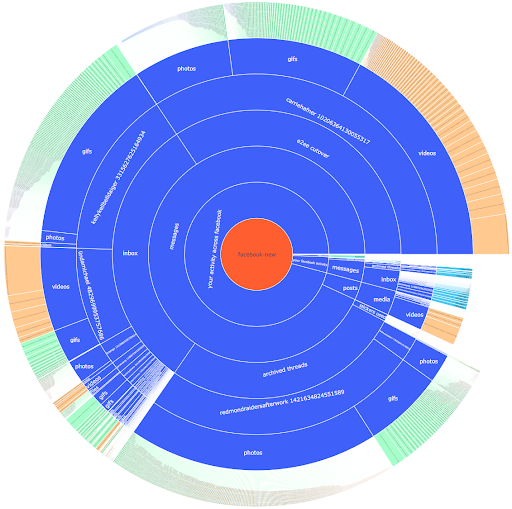
\includegraphics[width=0.5\textwidth]{img/fsb.png}
    \caption{Filesize Sunburst, generated from Peter's data.}
    \label{fig:fsb}
\end{figure}

Fig.~\ref{fig:fuy} demonstrates an example of the Facebook Use by Year graph. This shows a user's activity over time, represented by a three-dimensional stacked area plot from 2010 to 2024. The graph shows data points categorized into messages, likes/reactions, comments, and posts. The z-axis is presented on a logarithmic scale to enhance the visibility of categories with lower magnitudes of data, such as the posts and comments. 

\begin{figure}[htbp]
    \centering
    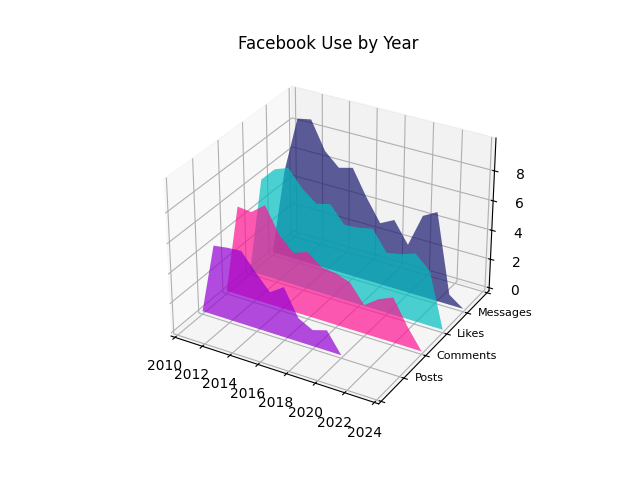
\includegraphics[width=0.5\textwidth]{img/fuy.png}
    \caption{Facebook Use by Year, generated from Peter's data.}
    \label{fig:fuy}
\end{figure}

Another visualization from the Facebook activity feature is the Message Sentiment Scatter. Facebook stores all of the messages and posts ever created by its users, and this visualization shows the messages sent over time. A sentiment analysis technique was used to grade every message on a scale of -1 to +1 based on whether the message was positive or negative. Fig.~\ref{fig:ssp} below demonstrates an example of this visualization, showing all messages sent by the user along with the sentiment of each. This specific example demonstrates a frequent use of Facebook during the early 2010s, when the user first made their account, a period of less frequent use afterwards, then an uptick in usage starting around 2021. In this specific example, the messages are slightly positive on average, but there's a large range across the whole plot.

\begin{figure}[htbp]
    \centering
    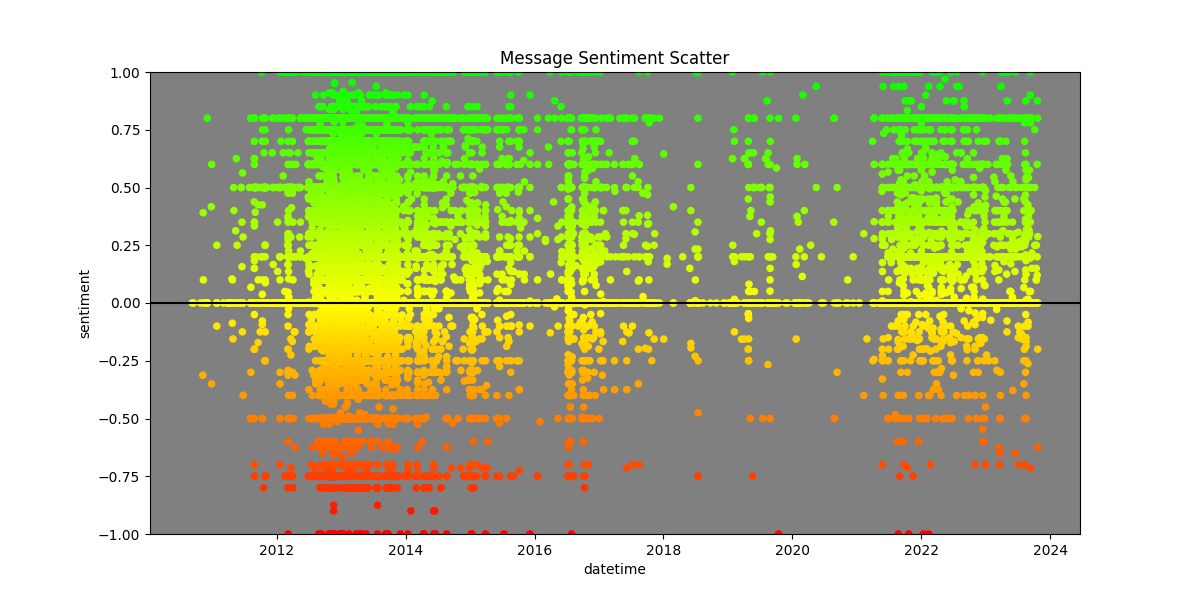
\includegraphics[width=0.5\textwidth]{img/mss.png}
    \caption{Message Sentiment Scatter, generated from Peter's data.}
    \label{fig:ssp}
\end{figure}

To further explore the data Facebook collects on its users, the next feature was created to visualize the data gathered from external sources, represented in the 'Off Facebook Activity' directory. Fig.~\ref{fig:ofa} represents the most visited sites reporting to Facebook. The bar charts highlight some surprising insights into data communication with Facebook. Notably, Discord, a platform often perceived as less invasive in terms of data sharing, dominates my online activity, suggesting a frequent but unexpected level of data exchange with Facebook. This revelation is intriguing given Discord's community-oriented and privacy-aware undertone. Conversely, AliExpress, which might typically be expected to have extensive data sharing practices due to its commercial nature, shows a lower than anticipated visibility.

\begin{figure}[htbp]
    \centering
    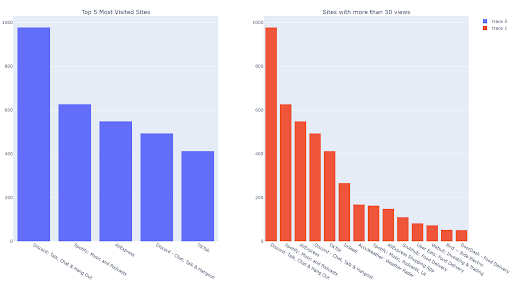
\includegraphics[width=0.5\textwidth]{img/ofa.png}
    \caption{Top 5 Most Visited Sites and Sites with more than 50 views, generated from Noah’s data.}
    \label{fig:ofa}
\end{figure}

To further illustrate the data collected by Facebook, IP logs were analyzed. Fig.~\ref{fig:ipl} below shows a screenshot of the visualization detailing the geographical locations for logged activity on Facebook's platform. Generally the data points seem to be accurate, but there were a handful of anomalies noted in each of the analyzed data sets. In this figure, it is clear that most of the points were in the Bellingham and New York areas, however the points in Eastern Washington, California, and New Hampshire were not locations visited during the analyzed time period.

\begin{figure}[htbp]
    \centering
    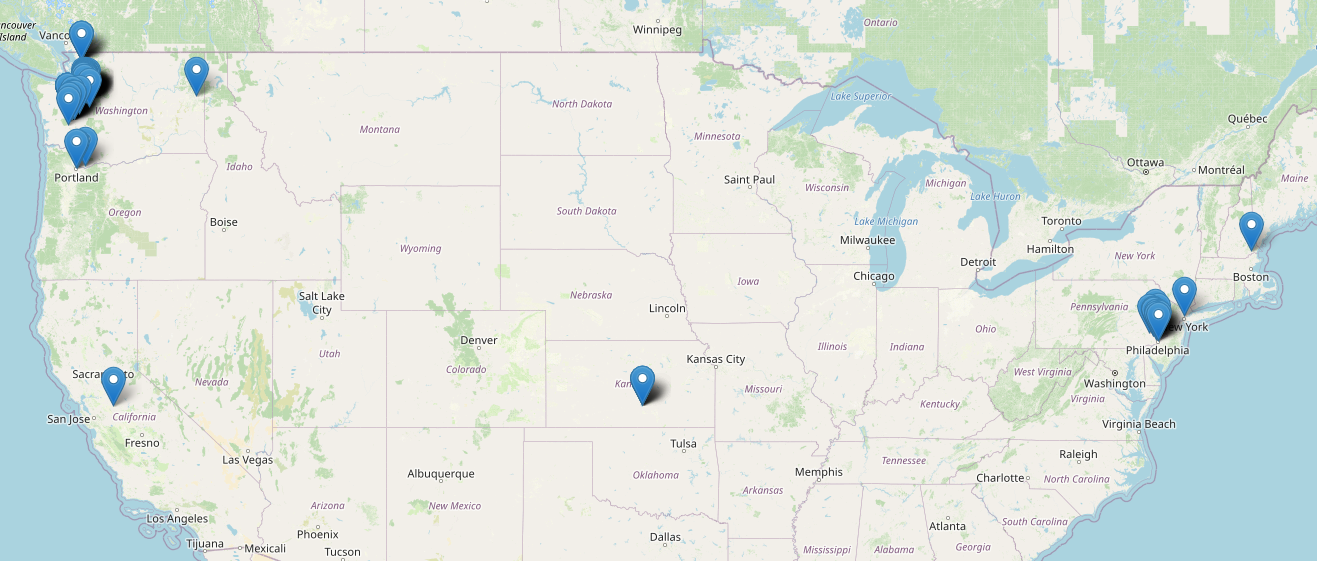
\includegraphics[width=0.5\textwidth]{img/ipl.png}
    \caption{IP Locations, generated from Carter's data.}
    \label{fig:ipl}
\end{figure}

Fig.~\ref{fig:ntf} shows an example of the notifications feature. Notably, the data points only represent the 30 days or so prior to the download. In this example, most of the data points appear on weekends. This is because the user is tagged in photos by his family on weekends, and generally interacts with social media more the weekend due to schoolwork during the week.

\begin{figure}[htbp]
    \centering
    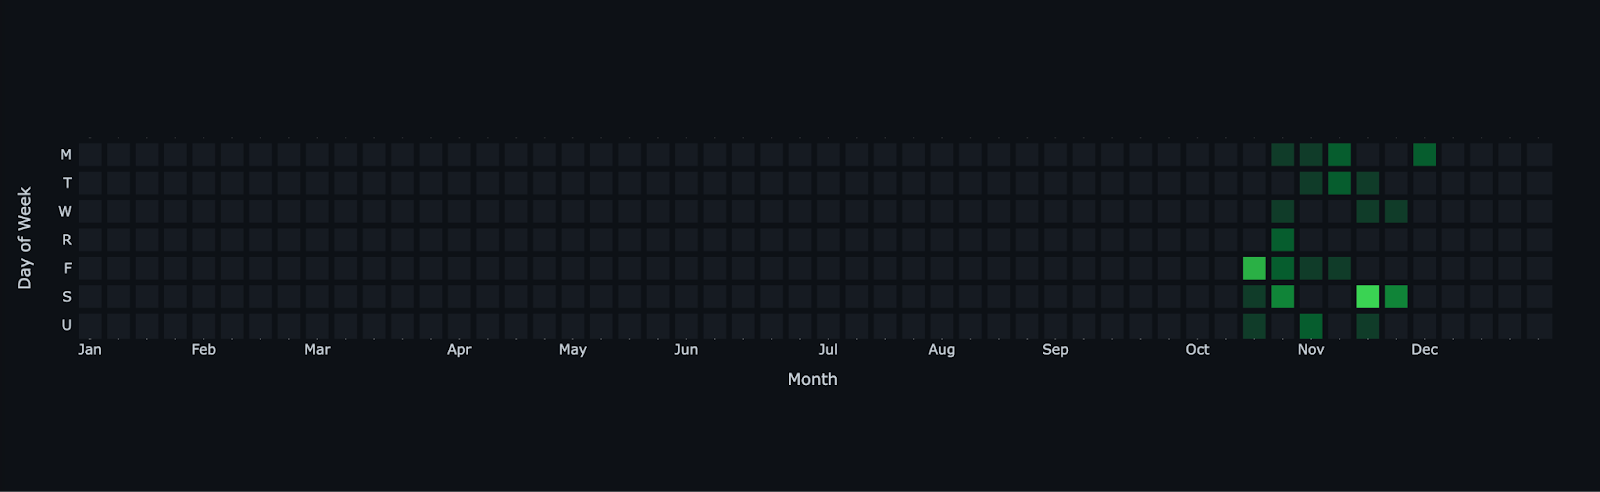
\includegraphics[width=0.5\textwidth]{img/ntf.png}
    \caption{Notifications, generated from Trevor's data.}
    \label{fig:ntf}
\end{figure}

Finally, the last topic analyzed is the ads interests and topics. To visualize this, the first image in a google search was pulled for each data point in the ads interests and topics files. This data shows the topics that Facebook thinks its users are interested in. Fig.~\ref{fig:tps} is an example of one of these generated visualizations. Interestingly, most of the represented images are not actually subjects that the user is interested in. This was consistent with the rest of the users, with some topics having been relevant at some point in the past and some topics never having been relevant at all.

\begin{figure}[htbp]
    \centering
    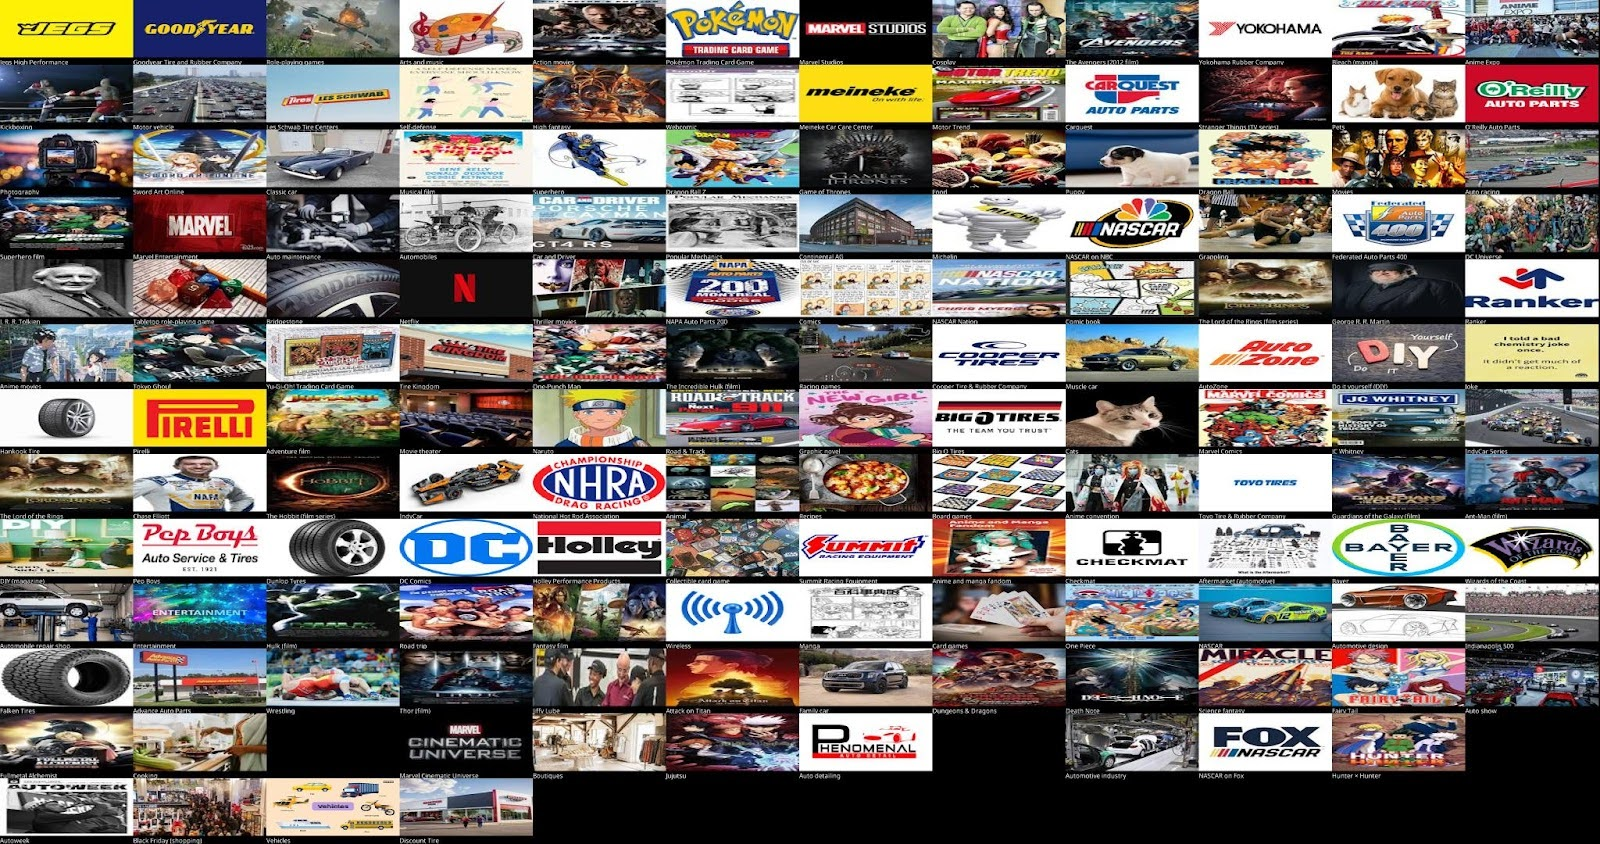
\includegraphics[width=0.5\textwidth]{img/tps.png}
    \caption{Ads Interests, generated from Carter's data.}
    \label{fig:tps}
\end{figure}

\section{Reflection} \label{RE}
The original goal of creating visuals for the general public to understand their data was fulfilled. Over meetings with the client across three quarters, more specific goals were explored, which became out of scope for the project due to time, current understanding and skills, or financial funds.

Each of our group members achieved their own personal goal and aspect to the project. Carter initially worked with the address book and friends list files before determining that the data collected was not visually interesting. Carter then moved on to working with the topics and ads interests files. Unfortunately, the topics file was removed from the Facebook data download around January 2024. Carter worked on creating the front facing website for the project. Trevor worked on plotting ip addresses and visualizing recorded ip addresses over time of use on Facebook. Trevor finalized on a map using the python folium library to plot the longitude and latitude with the help of MaxMind DB. Peter worked on analyzing activity across facebook via messages, posts, comments, and reactions. Sentiment analysis was run on these activities to gain further insight into how the user interacted with the platform, especially to show trends over time. Initially, Noah assembled a flexible json to csv converter, but it was ultimately depreciated due to runtime concerns. He then pivoted to creating the sunburst representation of the directory structure.

One of the biggest challenges we faced during project management was merging all the branches into one main branch. As a group, it became difficult because we initially worked in Jupyter notebooks, then needed to transition into an object-oriented Python script. We also encountered runtime issues with looping through the data, due to implementing RateLimiter when using APIs to avoid being whitelisted and receiving errors. This issue was resolved with the help of Piper Wolters and the introduction of multiprocessing, which greatly reduced our runtime.

\section{Conclusion} \label{CO}
After finishing the project, a key finding that became a challenge as a group was that Facebook upkeeps and changes the structure of their json files which became an issue for our implementation. There appears to be some intentional obfuscation of the data from Facebook's end here, as the documentation is minimal and the format/structure changes somewhat frequently. The project was able to achieve its goals by generating visuals for the general public in pursuit of understanding one's digital footprint. This project includes a website with instructions on how to use the program, and how to download one's data from Facebook.

The potential impact of this project could provide insight to active, consistent users. The visuals allows users of all ages to unravel the mystery of their collected data from Facebook.

To avoid discrepancies future proofing was needed to be implemented since the parsing of files could be changed in the future. For future work, this project was documented enough so that another group can easily pick up the project. This project needs to be presented formally since it will be presented in a conference in Europe with all of our findings and the package of our code. 


\section*{Acknowledgments}

Among others, we would like to thank Dr. Brian Hutchinson and Piper Wolters for their guidance and support throughout this project.

\printbibliography
\end{document}
